\def\year{2015}
%File: formatting-instruction.tex
\documentclass[letterpaper]{article}
\usepackage{aaai}
\usepackage{times}
\usepackage{helvet}
\usepackage{courier}
\usepackage{url}
\usepackage{array}
\usepackage{graphicx}
\usepackage{amsmath}
\usepackage{graphicx}
\usepackage{subfig}
\newcolumntype{L}[1]{>{\raggedright\let\newline\\\arraybackslash\hspace{0pt}}m{#1}}
\newcolumntype{C}[1]{>{\centering\let\newline\\\arraybackslash\hspace{0pt}}m{#1}}
\newcolumntype{R}[1]{>{\raggedleft\let\newline\\\arraybackslash\hspace{0pt}}m{#1}}
\newenvironment{blockquote}{%
  \setlength{\parskip}{.5em}
  \par%
  \small
  \medskip
  \leftskip=3em\rightskip=3em%
  \noindent\ignorespaces}{%
  \par\medskip}
\newcommand{\specialcell}[2][l]{%
  \begin{tabular}[#1]{@{}l@{}}#2\end{tabular}}
\frenchspacing
\setlength{\pdfpagewidth}{8.5in}
\setlength{\pdfpageheight}{11in}
\pdfinfo{
/Title Pre-orders or Philanthropy: An Analysis of Altruism on Kickstarter
/Author Jack Hessel
/Keywords X,Y,Z}
\setcounter{secnumdepth}{0}  
 \begin{document}
% The file aaai.sty is the style file for AAAI Press 
% proceedings, working notes, and technical reports.
%
\title{Pre-orders or Philanthropy: An Analysis of Altruism on Kickstarter and Other Crowdfunding Sites}
\author{Jack Hessel}
\maketitle
\begin{abstract}
\begin{quote}
In this study we conduct several experiments related to altruistic behavior on Kickstarter and other crowdfunding sites. This realm has been relatively unexplored in previous work, which is surprising given that roughly 20\% of all backing money on Kickstarter is donated. Because previous studies sugguest that lingustic features are very important to requests made online, language is a focal point of our analysis. We first find that Kickstarter exists in a lingustic realm somewhere between pure altruism and pure commericalism. Next, we find that useful information about the sequential nature of requests can be learned in an unsupervized fashion. Also, we find that linguistic features of Kickstarter campaigns are able to predict whether or not projects attract above-average levels of prosocial activity. Finally, and most surprisingly, we find that failing projects are acutally more likely to recieve altruistic donations, sugguesting the existance of a subset of users who frequently give small amounts of money to failing projects and request no rewards in return.
\end{quote}
\end{abstract}

\section{Introduction}

In recent years, crowdfunding websites have emerged as a popular method of fundraising for individuals looking to promote their ventures to online communities. The most popular of these sites, Kickstarter, provides a venue for entrepreneurs to connect with individuals who might be interested in financially supporting their project ideas, which range from artistic endevours to technology startups. To date, over \$1.4B has been invested in Kickstarter projects from more than 7.4M unique backers resulting in over 73K successfully funded projects. \footnote{ \url{www.kickstarter.com/help/stats}} Each project is associated with a set of creator-defined rewards that donors can choose from. Often, these rewards constitute pre-orders of a product that the project aims to bring to market.

We argue that crowdfunding sites similar to Kickstarter occupy a unique space between a realm of pure salespersonship and a realm of pure altruism. A project that illustrates that Kickstarter is not purely altruistic nor purely commerical is ``Juicies.''\footnote{\url{http://tinyurl.com/juiciesproject}} In this project, the creators successfully attempted to create a company that sells multi-colored charging cables for various mobile devices, and offered cable preorders as rewards. The basic cable was associated with two rewards, one costing the suggested retail price of \$20, and the other charging users to ``pay what you can'' for the same cable costing \$1. While over 1K pay-what-you-can rewards were claimed, the \$20 reward was claimed 280 times. Users voluntarily paying more for an identical product sugguests that Kickstarter is not a community solely focused on commercialism. This observation matches previous work which sugguests that people use crowdfunding tools for reasons other than personal gain \cite{van2011fighting}.

\begin{table*}[t]
\centering
\scriptsize
\begin{tabular}{|*{12}{c|}}  % repeats {c|} 18 times
\hline
\multicolumn{6}{|c}{GoFundMe vs. Kickstarter} & \multicolumn{6}{|c|}{Amazon vs. Kickstarter} \\ \hline
\multicolumn{2}{|c}{Unigrams} & \multicolumn{2}{|c}{Bigrams} & \multicolumn{2}{|c}{Trigrams} & 
\multicolumn{2}{|c}{Unigrams} & \multicolumn{2}{|c}{Bigrams} & \multicolumn{2}{|c|}{Trigrams} \\ \hline 
Unigram & Z & Bigram & Z & Trigram & Z & Unigram & Z & Bigram & Z & Trigram & Z \\ \hline
the & -77.52 & of the & -42.74 & be used to & -9.05 &
we & -685.35 & will be & -367.20 & be able to & -141.92 \\\hline
of & -42.74 & to create & -20.17 & some of the & -8.26 &
i & -525.09 & we are & -256.59 & thank you for & -112.63 \\\hline
new & -26.01 & on the & -19.96 & will be a & -6.25 &
will & -514.99 & we have & -218.54 & a part of & -94.38 \\\hline
show & -25.24 & about the & -16.48 & be used for & -6.07 &
our & -501.84 & we will & -193.24 & in order to & -93.87 \\\hline
create & -23.99 & and the & -15.65 & to make the & -6.02 &
be & -356.80 & thank you & -186.89 & to make this & -92.88 \\\hline \hline

me & 80.57 & would be & 37.02 & take care of & 16.27 &
perfect & 64.77 & is the & 48.67 & the united states & 2.88 \\\hline
was & 82.01 & name is & 37.74 & to help with & 17.72 &
has & 73.00 & and is & 54.69 & is a great & 3.75\\\hline
am & 82.62 & family and & 40.60 & in need of & 19.04 &
with & 78.24 & with a & 56.31 & is one of & 27.54\\\hline
family & 98.81 & thank you & 41.80 & thank you for & 20.38 &
includes & 81.00 & has a & 56.71 & of the most & 30.88\\\hline
i & 136.42 & to help & 55.71 & friends and family & 27.25 &
easy & 82.72 & out of & 71.67 & one of the & 30.97 \\\hline
\end{tabular}
\caption{Summary of Bayesian analysis of language comparing Kickstarter to GoFundMe and Amazon. Negative Z-scores correspond to Kickstarter. Top ten most significant n-grams are presented. A full list of n-grams and z-scores is provided.\footnote{PUT LINK HERE}}
\label{tab:pairwise}
\end{table*}

Furthermore, in our dataset consisting of 45K completed Kickstarter projects, we are able to quantify the number of purely altruistic donation events and the total value given above and beyond the amount required for all reward claims. Of the roughly 3.4M donation events, about 360K (10.59\%) resulted from users who willingly opted to recieve no reward. Of the roughly \$246M pledged in our dataset, over \$53M (21.59\%) was given altruistically.

The community and language of Kickstarter have been studied previously. Mitra and Gilbert analyze the language that predicts successful Kickstarter projects \cite{mitra2014language}. When compared their baseline regression trained on a set of language-indepedent set of project features, their final classifier, which includes binary n-gram indicator variables, is able to classify projects 15\% more accurately, resulting in a 97.8\% correct prediction rate in a 10-fold cross validation setting. Similar analyses that do not take language fully into account are not able to achieve such predictive accuracy. Studies that use of minimal textual information in conjunction with baseline project features are able to learn classifiers that reach 68\% accuracy using information available at launch time \cite{greenberg2013crowdfunding}. Even using post-launch information, however, does not improve accuracy as much as accounting for language; 85\% accuracy is achieved using information available after 15\% of the duration of the campaign has expired \cite{etter2013launch}. Furthermore, lingustic factors have been shown to effect the quality and time-to-response of questions posed in an online community \cite{teevan2011factors}. These findings sugguest that language is very important on Kickstarter and, more generally, in online communities as a whole, which is a primary motivation for making it a focus of our analysis.

Altruism in online communities has also been previously studied. Althoff et al. examine a purely altruistic community wherein users request and provide free pizza to and from other community members \cite{althoff2014ask}. An advantage of their dataset is that all their request are purely altruistic, and are made for the same service, though the total donation value of their dataset is lower than that presented here. Previous work on Kickstarter has also demonstrated that users are more likely to donate to campigns as time is winding down and the project has not yet met its goal, which is an arguably altruistic behavior \cite{kuppuswamy2013crowdfunding}.

These observations and previous work motivate our research questions: how does the language used on Kickstarter differ from the language used in a purely commercial setting? Or a purely altruistic setting? What types of Kickstarter projects are donated to altruistically? Does the language of a project description predict the donation behavior of backers?

\section{Primary Dataset}
Our dataset consists of 45810 completed Kickstarter projects, the URLs of which were originally collected by AppsBlogger.com. The projects in our data were all active between April 2009, the earliest start date, and August 2012, the latest end date. Every Kickstarter project has an associated HTML page, which we parse using the popular HTML parsing library Beautiful Soup 4\footnote{\url{http://www.crummy.com/software/BeautifulSoup/}}. Each project's page contains information about the project such as its title, its description, the rewards (with associated cost, number of backers who have claimed that reward, and a description), the FAQ section, the total number of backers, and the total amount of money raised. This information served as the basis of our analysis.

Kickstarter projects are also associated with a single category. The category of a Kickstarter project is used by the site to index campaigns and to help users find projects of a specific type. While some of these categories are ``main'' categories (13/49) most are ``subcategories'' that have a corresponding main category. In most cases, we treat all categories as equivalent, irrespective of whether or not it is a sub or a main.

In all of our analyses that use text data, we preprocess by removing punctuation from strings and converting all characters to lower case, though we do not discard stop words. In general, we are interested in unigrams, bigrams, and trigrams, and tokenize after these preprocessing steps.

\section{Kickstarter vs. GoFundMe and Amazon}
What language used on Kickstarter is altruistic? What language used on Kickstarter is commercial? To address these questions, it might be possible to derive stringent definitions of altruism and salespersonship. However, for our analysis, we resort to a more objective analysis by incorporating two additional data sets, one from Amazon and one from GoFundMe.

Amazon is a very popular online marketplace, where users can purchase items from a wide range of categories. Each product is associated with a description and and a set of categories. Our dataset consists of just over 1M Amazon product descriptions \cite{mcauley2013hidden}. We consider Amazon product descriptions as a gold standard purely commercial dataset.

On the other hand, GoFundMe is a crowdfunding site similar to Kickstarter, but campaigns are generally more focused on charitable/personal ventures. For instance, a popular category on GoFundMe is ``Medical,'' wherein users create pages to raise money for medical expenses for family and friends. Our dataset consists of 7.7K GoFundMe project descriptions scraped in November 2014. In contrast to Kickstarter, in a vast majority of cases GoFundMe contributors don't have the option to select compensentory rewards, and we therefore regard our GoFundMe data as requests for purely altruistic actions.

To compare the language used on Kickstarter to purely commercial and purely altrustic pitches, we adopt a Bayesian approach that has previously been successful in comparing the language used by two political parties on a specific issue \cite{monroe2008fightin}. In a general sense, this model has been used to compare word usage between two related corpora in a princpled way. Under the model, language is modeled as a ``bag of words'' represented by a multinomial distribution over vocabulary items. For the two corpora in question, we assume that their language distributions are drawn from a Dirichlet prior. Though it is possible in this scenario to encode useful information in the prior, we find it sufficient to utilize an uninformative prior and set our Dirichlet hyperparameter to be $\alpha=.01$. Assuming this language model, it becomes possible to compute approximate differences in vocabulary usages, and approximate variances of those differences.

In order to use this model, one must first define a vocabulary. Because we are interested in general language rather than specific subject matter, we apply a cross-categorical filtering scheme in an attempt to control for topic. Recall that in each of our datasets, documents are associated with one or more categories. In a first attempt to control for topic, we first applied a filter that removed all n-grams that didn't appear in all categories at least once. We found this simple filtration scheme to be inadequate -- the words ``book,'' ``publisher,'' and ``author,'' for instance, appear very frequently in the Amazon dataset because about 78\% of the products in the Amazon dataset are tagged under the Book category.

To apply a more stringent topic controlling filter, after removing n-grams that don't appear in all categories, for each n-gram $n$, we compute the intra-category document frequency denoted $f_n^c$ for all categories $c$ where $f^n_c$ is the average number of times $n$ appears in documents within category $c$. We then compute the ``normalized width'' $w_n$ for n-gram $n$ as...

\begin{equation} \label{eq:width}
w_n = \frac{\max\limits_{c'}f_n^{c'} - \min\limits_{c'}f_n^{c'}}{\max\limits_{c'}f_n^{c'}}
\end{equation}

The intuition behind normalized width is as follows -- if a word appears in all categories with roughly the same frequency, the normalized width will be small. If a word appears very frequently in a single category, the normalized width will be large. After computing this statistic for all n-grams, we discard the 10\% of n-grams with highest normalized width. This two-part filtration scheme is applied to all three datasets, and to derive our final vocabulary we take a 3-way intersection of the resulting topic-controlled features from Kickstarter, Amazon, and GoFundMe. The final vocabulary contains 2077 n-grams. The results of these analyses are summarized in Table \ref{tab:pairwise}.

These rankings clearly illustrate the commecial language used on Amazon and the altruistic language used on GoFundMe, when compared to Kickstarter. For instance, the most Amazon-like unigrams, ``easy,'' ``includes,'' ``with,'' ``has,'' and ``perfect,'' are highly sales oriented, whereas the most Kickstarter-like n-grams are more focused on personal appeals and promise of future improvement. Conversely, even a coursory examinination of the trigrams in the GoFundMe versus Kickstarter analysis reveals clear differences in lingustic content. Project curators in the more altruistic setting are clearly more focused on personal appeals when compared to Kickstarter.

To emperically analyze these n-gram comparisons, we first rank the n-grams in each experiment by their z-scores and compute Kendall's tau correlation between the Kickstarter vs. Amazon and Kickstarter vs. GoFundMe analyses. The intuition behind this comparsion is as follows: if Kickstarter is more altruistic than Amazon, but less altruistic than GoFundMe, then we would expect altruistically-associated n-grams to be on opposite ends of each ranking. This phenomenon occurs for the z-scores of n-grams like ``friends and family'' (-48.86 to 27.24) ``thank you for'' (-112.63 to 20.38) and ``love'' (-75.63 to 23.83) as one might expect, but does it happen in general?

For all 2077 n-grams, we observe a statistically significant negative correlation between the rankings ($\tau = -.035, p = .016$). In addition, we compute rankings and correlation statistics for our 1119 unigrams, 1101 bigrams, and trigrams seperately. As we shift our focus from unigrams ($\tau = -.024, p = .23$) to bigrams ($\tau = -.038, p = .061$) to trigrams ($\tau = -.041, p < .01$) the negative correlation between the rankings both becomes greater and more significant. This is likely because more lingustic signal can be carried by phrases of increasing length.

Overall, we argue this analysis demonstrates that discourse on Kickstarter is neither entirely Amazon-like, nor entirely GoFundMe-like, but rather lies in its own lingustic regime at the intersection of altruism and commercialism.
\section{What do Altruistic Requests Look Like?}

\begin{table}
\centering
\footnotesize
\begin{tabular}{|l|L{4cm}|}
\hline
Number of Sentences & Top 3 4-grams \\\hline
178 & \specialcell{`would be greatly appreciated'\\`as you can imagine'\\`donation is too small'}\\\hline
254 & \specialcell{`thank you for your'\\`thank you so much'\\`for taking the time'}\\\hline
356 & \specialcell{`to be able to'\\`not be able to'\\`will be able to'}\\\hline
192 & \specialcell{`to go to the'\\`to the er and'\\`back to the hospital'}\\\hline
275 & \specialcell{`we are asking for'\\`are asking for help'\\`our friends and family'}\\\hline
243 & \specialcell{`in the middle of'\\`the middle of the'\\`a \# year old'}\\\hline
272 & \specialcell{`was diagnosed with stage'\\`diagnosed with stage \#'\\`she was diagnosed with'}\\\hline
255 & \specialcell{`is one of the'\\`one of the most'\\`find it in your'}\\\hline
181 & \specialcell{`will be greatly appreciated'\\`will be a long'\\`long road to recovery'}\\\hline
224 & \specialcell{`to help with medical'\\`will go directly to'\\`to raise money for'}\\\hline
104 & \specialcell{`he is able to'\\`he is in a'\\`fighting for his life'}\\\hline
\end{tabular}
\caption{11 content clusters derived from the content model.}
\label{tab:contentmodel}
\end{table}

\begin{figure}
\centering
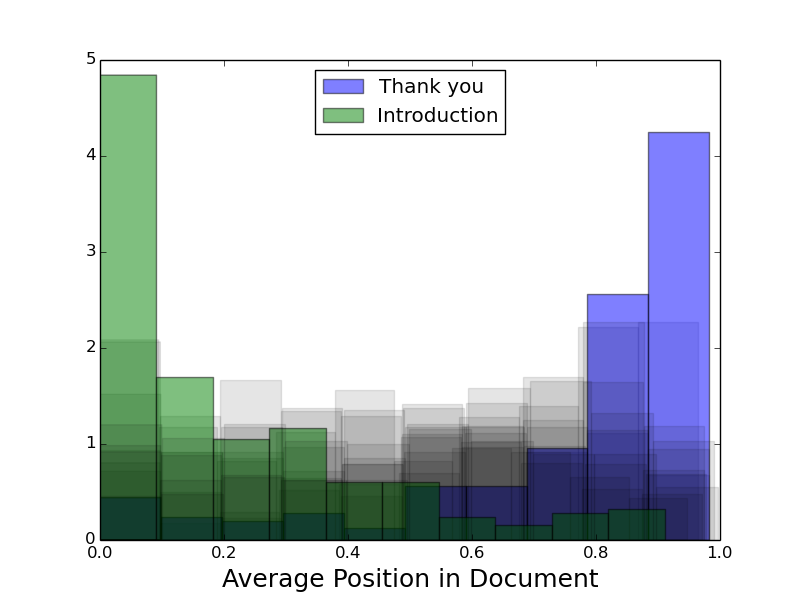
\includegraphics[width=.45\textwidth]{figures/docpos.png}
\caption{The average document position of sentences in the ``Introduction'' and ``Thank you'' clusters. It's clear that, in general, sentences related diagnoses occur at the beginning of documents, where as thank you's are expressed at the end. Similar histograms for all other clusters are superimposed in black for comparison.}
\label{fig:docpos}
\end{figure}

To analyze the sequential structure of altruistic requests in a crowdfunding setting, we run a case study on a subset of data utilizing a content model \cite{barzilay2004catching} to produce a sentence clustering. A content model is an unsupervized learning algorithm that operates on the sentence level, takes information order into account, and learns transition probabilities between sentence types. Here we provide a brief overview of the content model algorithm; for a fuller description, consult the original paper.

The goal of a content model is to learn a set of sentence clusters utilizing ordering information. Given a set of $N$ documents where document $n$ has $s_n$ sentences, sentences are first clustered into $k$ groups according to bigram features using complete-link clustering with a cosine distance metric. After sentences are clustered into these groups, we merge all clusters smaller than some threshold into an ``etcetera'' cluster. This etcetera cluster is a unique feature of the content model that allows it the flexibility to assign sentences that otherwise don't fit into an ``other'' cluster. After this merging process, we are left with $m$ clusters. 

For each of the resulting non-etcetera clusters, we train a smoothed bigram language model which is able to assign probabilities to input sentences. For the etcetera cluster, we train a ``complentary'' language model which assigns high probability to sentences that all other language models assign low probability to.

After training these language models, we now treat each clustering as a state in a Hidden Markov Model, and all input documents as emissions from that Hidden Markov Model. We are able to compute the Viterbi path for each document, and we re-cluster sentences based on these most-likely paths. Finally, we retrain each of the language models based on the new clustering. This process of re-clustering, computing Viterbi paths, and re-training language models in an expectation 
maximization-like fashion is executed until convergence or a maximum number of iterations is made. 

In accordance with the reccomendations of the original authors, we attempt to map all named entities to a ``NAME'' token and all numbers to a ``NUM'' token. We use the default NLTK\footnote{\url{http://www.nltk.org/}} named entity recognizer to identify tokens to be mapped to ``NAME,'' and we map any token that parses to a float without error to ``NUM.''

We apply the content model to a small subset of the GoFundMe corpus (460 documents with a total of 7K sentences) corresponding to the campaigns listed in the ``Medical'' category. We utilize 11 content clusters and 1 etcetera cluster in our model. Though the original literature sugguests a larger number of clusters (30+) we opt for a smaller, interpretable analysis because our resulting model was not used for any information ordering or information extraction tasks, as in \cite{barzilay2004catching}. After our expectation maximization converged after nine iterations, we were left with the order-aware sentence clusters displayed in Table \ref{tab:contentmodel} (etcetera cluster omitted).

Clearly, there are clusters of all sorts that represent different pieces of a generalized plea for help with medical expenses. One interesting cluster is the ``Ability'' cluster, which contains 356 sentences. Describing in detail a lack of ability is likely to elicit empathetic feelings from a reader, and, according to the well-supported empathy-altruism hypothesis, empathetic feelings are very likely to lead one to purely altruistic behavior, such as donating on a crowdfunding site \cite{batson1988five}.

Content models carry with them the advantage that sentences with disjoint bigram features may be clustered together based on the order of sentences after EM is applied. For instance, ``your contributions big or small are greatly appreciated,'' ``as a family we thank you,'' and ``god bless you have a wonderful day'' are clustered together. Despite the three sentences having disjoint bigram features and being entirely dissimilar according to the original, order-unaware clustering scheme, the content model is able to discern that the three likely have similar meaning based on their placement in documents relative to other sentences.

For the remaineder of this analysis, we are going to focus on the cluster containing 254 sentences (dubbed the ``Thank you'' cluster) and the cluster containing 272 sentences (dubbed the ``Introduction'' cluster). Though there are many interesting things that can be learned from the transition probabilities output by the content model, the most interpretable fact is illustrated in Figure \ref{fig:docpos}. This figure shows the distribution of normalized sentence position of each cluster in the sentences in the dataset. For a given cluster $c$, this statistic is defined as
\begin{equation} \label{eq:sentpos}
\sum\limits_{k \in \text{Occurances of $c$}} \frac{\text{Position of $k$ in containing sentence}}{\text{Length of sentence containing $k$}}
\end{equation}
While this result is somewhat unsurprising (situations are introduced before authors thank readers) it demonstrates that the content model is able to learn useful information about ordering in an unsupervised fashion, and that aspects of the sequential nature of altruistic requests are learnable by this method.

\section{Prediction of Altruism on Kickstarter}
\begin{table}
\centering
\begin{tabular}{|l|L{5cm}|}
\hline
Goal & Project funding goal (dollars) \\\hline
Featured & Project was selected by Kickstarter staff and advertised as such\\\hline
Duration & Project's duration (days) \\\hline
Num Levels & Number of reward types \\\hline
Minimum Pledge & Minimum pledge to get a reward (dollars)\\\hline
Video & Indicates whether or not the project has an associated video \\\hline
Num Updates & Number of ``updates'' projects owners have posted \\\hline
Num Comments & Number of user comments posted \\\hline
Facebook Connected & Indicates whether or not project owners have personal Facebook profiles associated with Kickstarter\\
\hline
\end{tabular}
\caption{Descriptions of the control features used in the regression tasks.}
\label{tab:controls}
\end{table}

How does altruism manifest on Kickstarter? When a user backs a project on Kickstarter (which is impossible to do anonymously) they are prompted to select a backer reward of value less than or equal to their donation amount. If a user does not want to claim a reward but, rather, donate altruistically, there exists an option that allows them to claim no reward. Because the total number of claims for each non-altruistic reward are displayed publicly on the project page along with the total number of backers (altruistic and non-altruistic alike) we are able to compute the total number of purely altruistic donation events for each project. Furthermore, the site allows for users to give an amount exceeding the cost of a given reward, so we are able to compute the total amount donated to a project above and beyond the amount required for all the posted reward claims. As previously noted, altruistic donation events constitute 10.59\% of all donation events and 21.59\% of all money donated in our dataset (over 53M dollars) was given away.

In a similar vein to \cite{mitra2014language} we define a binary altruistic response variable and train several logistic regression classifiers to predict that variable. The response variable is defined as follows: if a project recieves any donations and the proportion of altruistic donations it recieves exceeds $10\%$, we assign it to the altruistic group, otherwise, it is assigned to the non-altruistic group. We can interpret this binary variable as ``recieved more than an average number of altruistic donations.'' Defining this control variable partitions the dataset into 26733 altruistic projects and 19077 non-altruistic projects giving a constant prediction baseline of 58.34\% accuracy.

Out first regression task consists of a controls-only baseline. The set of control variables, which mostly mirrors Mitra and Gilbert's control set, consists of 49 binary variables, one for each Kickstarter project category (``Theater,'' ``Indie Rock,'' ``Open Software,'' etc.) and an additional 10 variables summarized in Table \ref{tab:controls}.

We use glmnet \cite{friedman2010glmnet} for our regression tasks. glmnet is a software package that implements cyclic coordinate decent and is capable of performing penalized regression tasks on highly sparse datasets. For our experiments, we utilize an $L_1$ (lasso) regularization term in an attempt to enforce sparsity and derive a parsimonious model. Furthermore, we set glmnet to perform 10-fold cross validation to search for the optimal regularization coefficient and prevent overfitting. In addition to training a model on all the data using cross-validation, as a seperate measure of model generalizability we also report test accuracy when spliting our data into a 40k project training set and a 5k project test set. Notably, glmnet purposefully does not report standard errors on resulting feature coefficients because the regularization process intorudces substantial bias into the regression process.

Using a model consisting of controls only, we achieve a cross-validation accuracy of 64.53\% (6.19\% improvement over constant prediction) and a testing set accuracy of 63.80\% (5.46\% improvement). The most important positive and negative predictive features were all Kickstarter categorical control variables. Dance, theater, public art, performance art, and classical music ($\vec{\beta} = \langle 1.84, 1.56, 1.24, 1.04, .930 \rangle$, respectively) were the categorical variables which were the strongest positive predictors, whereas board/card games, games, comics, video games, and product design ($\vec{\beta} = -\langle 1.64, 1.23, 1.02, .862, .795 \rangle$, respectively) were the strongest negative predictors. This result indicates that product category is the most important factor in determining if a project will recieve altruistic donations, and perhaps that projects in artistic categories are more likely to recieve such Kickstarter backing. This result is fairly unsurprising -- artistic endevours are generally regarded as intrinsically valuable to society, as evidenced by the existance of organizations like the National Endowment of the Arts which has, to date, awarded more than 5B dollars for artistic endevours\footnote{\url{http://arts.gov/about-nea}}. The negatively predictive categories tend to have concretely associated products with their projects (a video game, for instance) and backers likely pre-order instead of donate, in general.

The most important non-categorical positive predictor was having a video (binary variable, $\beta = .45$). On the other hand, being featured (binary variable, $\beta = -.183$) and having many comments on a project (interger variable, $\beta = -.00168$) were associated with less altruistic donations.

\begin{table}[t]
\centering
\begin{tabular}{|l|l|}
\hline
Positive Predictors & Negative Predictor \\
\hline
universitys, .377 & people that are, -.384 \\
the challenge of, .308 & we going, -.348\\
so exciting, .296 & with international, -.278\\
at the park, .293 & can walk, -.271\\
taken off, .292 & ground the, -.260\\
my senior, .284 & complement, -.259\\
whatever you can, .277 & get in on, -.253\\
to austin, .252 & 20 you, -.227\\
to maintain a, .243 & must make, -.217\\
500 you will, .238 & my website at, -.212\\
underserved, .232 & use one, -.209 \\
way your, .232 & other ways you, -.204\\
recipient of, .230 & so we know, -.193\\
small portion of, .226 & this project it, -.191\\
was chosen, .224 & and rare, -.188\\
\hline
\end{tabular}
\caption{The top 15 positive and negative lingustic predictors of the binary variable ``did this project recieve an above average proportion of altruistic donations'' in the controls + n-grams model.}
\label{tab:regression}
\end{table}

Does accounting for linguistic content of a project increase our predictive accuracy? Our textual features consist of binary indicator variables for unigrams, bigrams, and trigrams in the project descriptions, FAQ question/answers, and reward descriptions of our Kickstarter projects. We apply the same two-part normalized width filter that we use in our previous analysis to determine a set of topic-free n-grams, which forces selected n-grams to appear in every Kickstarter category and be relatively uniformly distributed between them (see Equation \ref{eq:width}). Applying this two-part filtration process on our Kickstarter dataset exclusively, we end up with 31281 filtered n-grams.

When we incorporate these particular lingustic features as binary indicator variables, our cross-validation accuracy increases to 67.02\% (2.49\% improvement over controls-only baseline) and our testing accuracy increases to 66.68\% (2.88\% improvement). The inclusion of lingustic features, therefore, causes our predictive accuracy to increase slightly but significantly.

Which n-grams are most predictive of greater-than-average donation frequency? The top 15 most significant positive and negative predictive lingustic features along with their corresponding regression coefficients are displayed in Table \ref{tab:regression}.

Are there any discernable patterns among these n-grams? An examination of the most positive-predicting linguistic features reveals that the advertisement of academic affiliation is a strong predictor of recieving a higher-than-average number of altruistic donations. The usage of ``universitys'' and ``my senior,'' in particular illustrate this point.
\begin{blockquote}
The AcaBelles are Florida State \textbf{University's} premier all-female a cappella group\ldots\par\noindent
This is \textbf{my senior} thesis film at Pacific Union College\ldots\par\noindent
\end{blockquote}
Based on this analysis, it's reasonable to state that the Kickstarter community is more likely to give to students without requesting any rewards in return.
Furthermore, positive sentiment and language that indicates the author's excitement about the project (``so exciting,'' ``the challenge of,'' ``taken off'') appears to positively predict donation.
\begin{blockquote}
This is about to get \textbf{so exciting} for the IBP! \par\noindent
We developed more recipes and got excited about \textbf{the challenge of} using whole foods\ldots\par\noindent
Podcasting has really \textbf{taken off} in the past year\ldots
\end{blockquote}
There are also some interesting patterns in the negatively-predicting n-grams. For instance, self-describing language appears to be a consistently negative predictor of altruistic donation. Though the usage of any short sequence of words can vary considerably, common usage of linguistic features like ``people that are,'' ``we going,'' ``so we know,'' and ``my website at'' demonstrate this phenomenon.
\begin{blockquote}
We are all likable and professional \textbf{people that are} trying to build something\ldots\par\noindent
How Are \textbf{We Going} to Pull This Off?\ldots\par\noindent
We have 7 or so years of experience building art ... \textbf{so we know} that we can make this project happen.\ldots\par\noindent
Please visit \textbf{my website at}\ldots
\end{blockquote}
Furthermore, it seems that lingustic features that make commands of backers (``get in on,'' ``must make'') are negative predictors of donations.
\begin{blockquote}
Participants \textbf{must make} their own travel/lodging arrangements\ldots\par\noindent
We only have room for 4, so \textbf{get in on} this quickly\ldots
\end{blockquote}
Finally, the portrayal of backer interaction with rewards also appears to have a significant effect on donations. For instance, ``recipient of'' is a strong positive predictor, whereas ``can walk'' is a strong negative predictor.
\begin{blockquote}
Depending on how much money you pledge you \textbf{can walk} away with something as small as a print\ldots\par\noindent
You will be the \textbf{recipient of} TWO different designs
\end{blockquote}

Overall, there are lots of interesting linguistic and psychological observations that can be made based on the most significant positive and negative language-based predictors. A full ordered list of n-grams along with associated regression coefficients is provided\footnote{PUT LINK HERE} if the reader is interested in performing their own analysis.
\begin{figure*}[t]
\centering
\subfloat{
  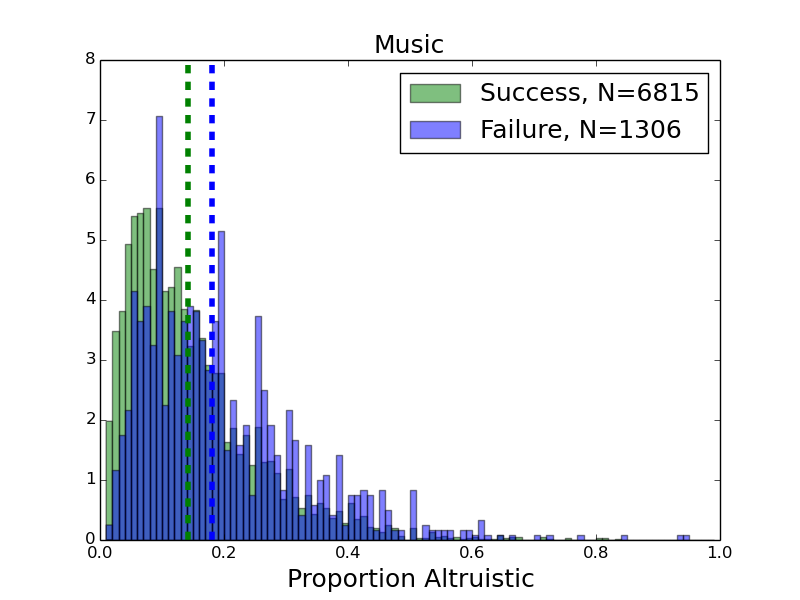
\includegraphics[width=.3\textwidth]{figures/Musicevents.png}
}
\subfloat{
  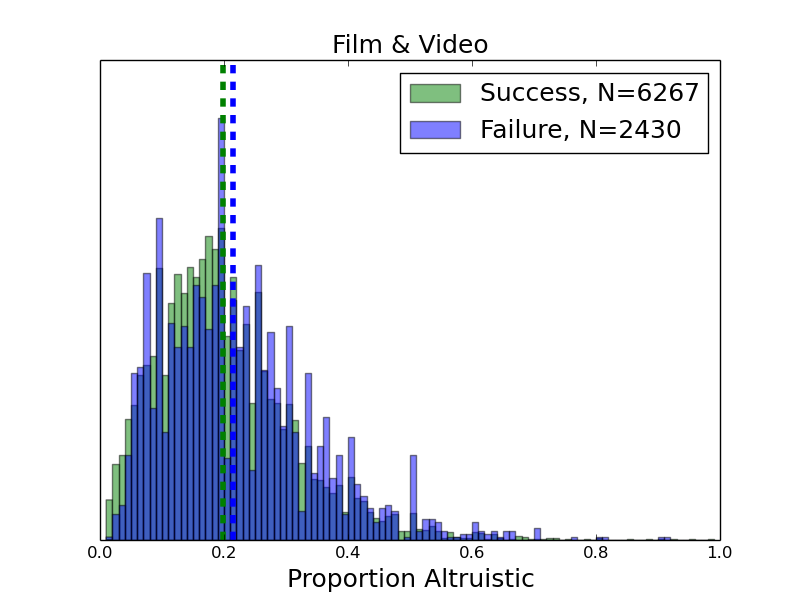
\includegraphics[width=.3\textwidth]{figures/FilmVideoevents.png}
}
\subfloat{
  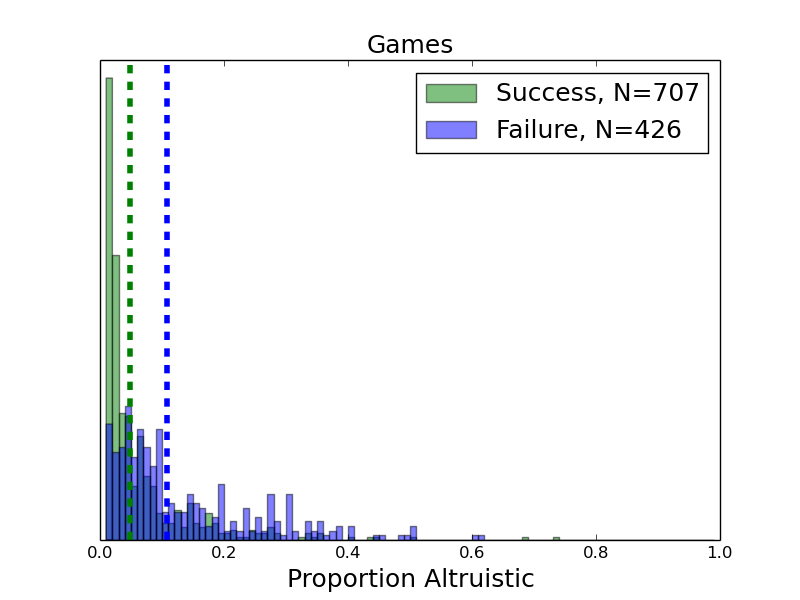
\includegraphics[width=.3\textwidth]{figures/Gamesevents.png}
}
\hspace{0mm}
\subfloat{
  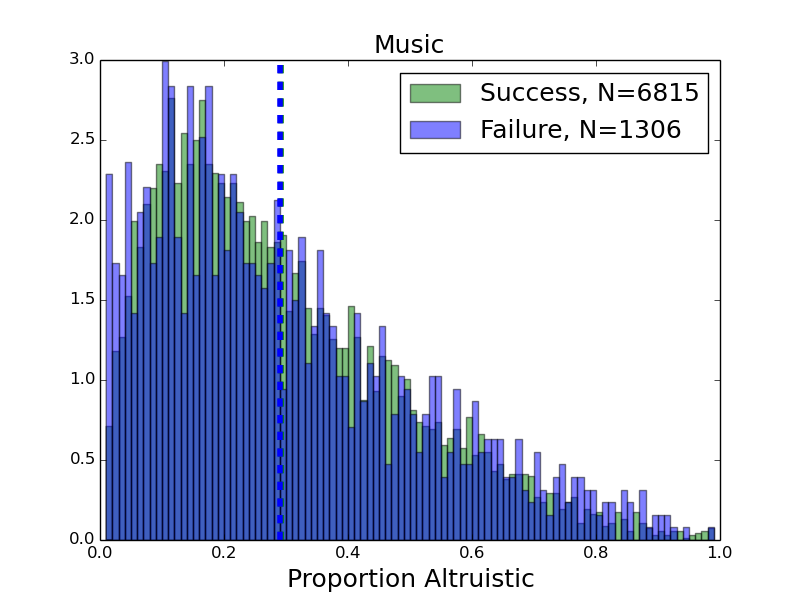
\includegraphics[width=.3\textwidth]{figures/Musicvals.png}
}
\subfloat{
  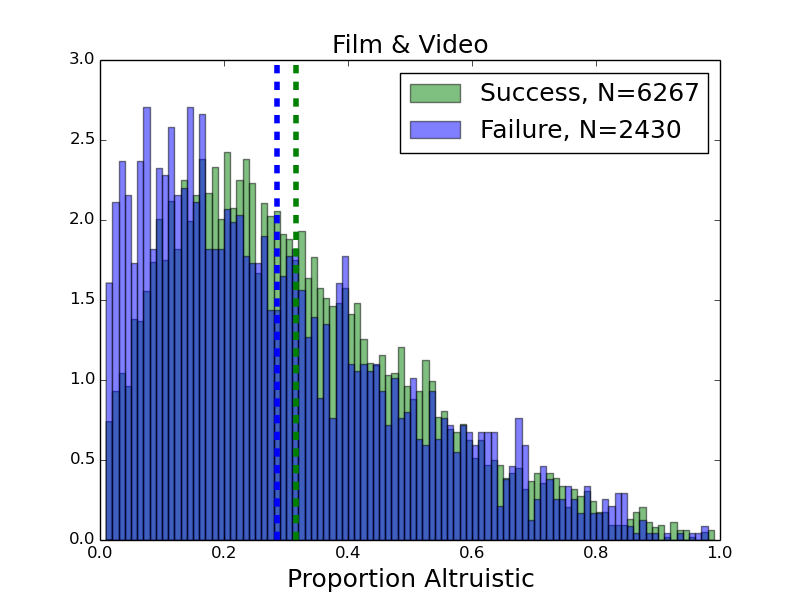
\includegraphics[width=.3\textwidth]{figures/FilmVideovals.png}
}
\subfloat{
  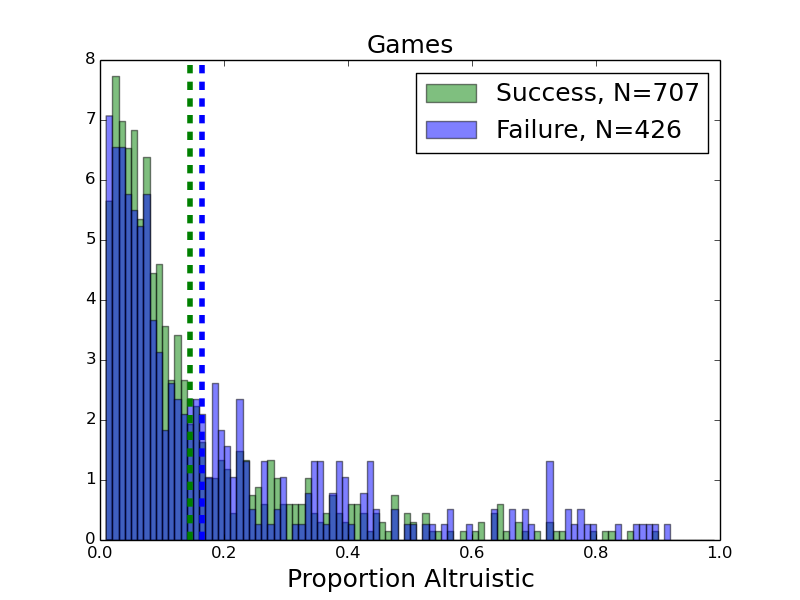
\includegraphics[width=.3\textwidth]{figures/Gamesvals.png}
}
\caption{Top row: event-based altruism distribution. x-axis represents the proportion of all donation events where contributors selected ``no reward'' when compared to all donation events for a project. Bottom row: dollar value-based altruism distribution. x-axis represents the proportion of all money raised that was given above-and-beyond the required value of the claimed rewards, when compared to the total amount raised for a given project. For both rows, dotted lines indicate means for successful and unsuccessful projects. The first two columns represent projects from the two most popular categories, ``Music'' and ``Film and Video,'' while the third ``Games,'' is included for topical contrast. All differences between the means in the graphs presented are significant at the 5\% level except for the ``Games'' and ``Music'' graphs in the second row.}
\label{fig:failsucc}
\end{figure*}
\section{Failing Projects, More Donations?}
What is the relationship between project success and the proportion of altruistic donations a project recieves? One might reasonably expect that successful projects, having higher quality pitches and commanding more donations on average, would also have a higher proportion of altruistic donations. In fact, the conclusions based on the analysis in this section find the \emph{opposite} to be true -- we find that, in fact, that there is a consistent negative association between project success and proportion of altruistic donations recieved.

To address this question, we first run a new lasso penalized regression task where predictive variables consist of the control variables highlighted in Table \ref{tab:controls} plus two additional binary variables, namely ``success,'' which indicates whether or not the funding goal of the project was reached, and ``numBackers,'' the total number of backers for a given project. The target of this new regression is the proportion of altruistic donations a project recieves. Because our target is a ratio that is highly sensitive to noise if the number of project backers is small, we restrict our consideration to the 30858 projects in our dataset with 10 or more backers (though the results presented here are robust to reasonable changes in this threshold).

Surprisingly, our resulting regression assigns negative weights to both our new predictive variables. With respect to the number of backers, the negative weight indicates that more popular projects are less likely to recieve altruistic donations, in general. More surprising, however, is that after controling for all variables in Table \ref{tab:controls} and project size, successful projects recieve \emph{less} altruistic donations than unsuccessful projects.

To further investigate this result, we split all projects with more than ten backers into the 13 main categories on Kickstarter\footnote{Our previous analysis mentioned 49 categories, but this division takes into account subcategories of the main categories. For this analysis, we use only the main categories.}. Next, we compute the distribution of two statistics for each category: the proportion of altruistic donation events (i.e. the number of times a backer selected the ``no reward'' option divided by the total number of backers) and the proportion of total project funding resulting from above-and-beyond contribution which is given by
\begin{equation} \label{eq:altruism}
\frac{\sum\limits_{x \in \text{ Rewards of $p$}} \text{Backers}(x) \cdot \text{Cost}(x)}
{\text{Amount Raised}(p)}
\end{equation}
for some project $p$.

For the event donation frequencies, there is a clear pattern: in 12 of the 13 Kickstarter categories (the exception being ``Food'') failing projects recieve a higher proportion of altruistic donations, on average. In seven of the thirteen categories, this result is significant at the 5\% level. For categories with large numbers of projects, this result is often highly significant. For instance, in the two most popular Kickstarter categories, ``Music'' and ``Film and Video,'' we observe a that failed projects recieve, on average, significantly more altruistic donation events (Student's t-test, $p<<.001$ in both cases). Sample plots of the event distributions are presented in the first row of Figure \ref{fig:failsucc}.

When we change the focus of our analysis from events to dollar values, however, this pattern becomes less apparent, or reverses altogether. In the ``Film and Video'' category, for instance, we observe a total reversal, a significant result ($p << .001$) that states successful projects receive more dollars altruistically than failed projects. In fact, over all categories all statistically significant results state that successful projects recieve more funding. In the ``Music'' category, however, the test statistic is close to zero, and the difference is no longer significant as it was in the event-based analysis. Sample plots of the dollar value distributions are presented in the second row of Figure \ref{fig:failsucc}.

What does this discrepency between events and dollar value mean? We suspect that the many significant results for our event-based analysis indicate that, indeed, failing projects recieve, on average, more altruistic donation events. However, the value of these donations is likely small, as many of these results don't hold when actual dollar values are considered.

We believe that this result sugguests the following scenario is common across many categories: a Kickstarter user observes that a project is failing and makes a small donation, but requests no reward. It has been shown that feelings of sympathy can elicit prosocial behavior, even if the interaction can be easily avoided, as it would be by anonymously closing a browswer window \cite{eisenberg1989relation}. If the cost of such an altruistic action is too high, however, it has a lower probability of being taken \cite{batson1983influence}. Though an assignment of altruistic donations to values directly would be valuable to our analysis, given the data that Kickstarter makes public, there is no way to directly compute the value of the altruistic donation events themselves, and we leave a more detailed analysis to future work on a seperate dataset.

Our hypothesis regarding low-cost donations fits very well into the framework established by previous psychological studies, assuming that feelings of sympathy are the driving force behind donation to failing projects. The existance and popularity of website entitled KickEnded\footnote{\url{http://kickended.com/about}} lends crediability to this theory. On KickEnded, finished Kickstarter projects with zero backers are archived so that they may ``live a second life... free from the pressure of money raising.'' The notion that commercial success does not equate to societial value is a highly sympathetic one. Though this evidence is rather indirect, it is a fairly strong indicator of the dynamics underlying our data.

Assuming our hypothesis is correct, several interesting questions arise. Who are these low-cost altruistic donators? Are their motiviations sympathetic, as the psychology literature and Kickended's popularity sugguest? Are there sub-communities of altruistic users? Are there community-derived benefits to making altruistic donations on Kickstarter? These specific questions would be best answered by Kickstarter users themselves; interesting future work might include questionaires sent out to a specifically targeted subset of users.

\section{Conclusion}

Here, we presented several analyses relating to altruistic behavior on crowdfunding sites with a focus on language. Our first analysis positioned Kickstarter somewhere between purely altruistic and purely commercial linguistic regimes. Next, as we examined the sequential structure of purely altruistic requests on GoFundMe and found that a content model was capable of learning an interpretable set of content-aware clusters that illustrate some of the stratigies authors use to ellicit donations. Then, noting that both event-based and amount-based altruistic activities can be determined based on the information presented on a Kickstarter page, we were able to extract the important linguistic features responsible for prediction of above-average donation levels. Finally, we made the surprising observation that failing projects tend to recieve more donation events, even after accounting for a wide range of control variables. This increased donation does not carry over to our amount-based analysis, however, sugguesting that failing projects recieve a large number of low-valued donations.

Overall, much more work could be done to analyze the dynamics of altruistic behavior on crowdfunding sites, and in ``mixed-altruism'' domains in general. As previously sugguested, one possible avenue for future research would be to identify and reach out to a subset of Kickstarter users that are likely to be responsible for frequent, low-valued donations given to failing projects. Another interesting avenue for exploration might be to identify and find similarities between other communities like Kickstarter.

Finally, our study has several limitations that could be overcome in future work. Many Kickstarter projects have very low valued ``dummy'' rewards that are functionally equivalent to altruistic donation (for instance, such a reward might cost \$1 and have the description ``Thanks!''). Its likely such rewards obscured some signal in our dataset. Furthermore, there are ``pie-in-the-sky'' type rewards that constitute altruism, as well (for instance, such a reward might cost \$10,000 and have the description ``Thank you! You will get a producer credit in our movie and our eternal gratitude''). In any case, a more careful consideration of rewards would be a well-suited topic for future work.

\section{Acknowledgements}

We would like to thank Eric Gilbert and Tanushree Mitra for providing their HTML scrape of Kickstarter, and all members of the Fall 2014 iteration of Cornell's CS6742 for the helpful conversations.

\bibliographystyle{aaai} \bibliography{refs}

\end{document}
